\documentclass{beamer}
\usepackage{graphicx}
\usepackage{xcolor}
\usepackage{listings}
\usepackage{hyperref}
\lstset{language=bash,
    morekeywords={in},
    basicstyle=\ttfamily,
    commentstyle=\color{red},
    keywordstyle=\color{blue},
    literate={\$}{{\textcolor{purple}{\$}}}1,
    moredelim=[s][\color{purple}]{\{}{\}},
    numbers=left,
    frame=single}
\usepackage{verbatim}

\usetheme{Madrid}
\AtBeginSection[]
{
  \begin{frame}
    \frametitle{Table of Contents}
    \tableofcontents[currentsection]
  \end{frame}
}

\begin{document}

\title{Intro to BASH}
\subtitle{Group 1}
\author{}
\date{First Year Bootcamp, 2016}
\frame{\titlepage}


\section{What are we bashing and why?}
\begin{frame}{What are we bashing and why?}
\begin{itemize}
    \item<1-> No violence involved, bash is a program!
    \item<2-> bash (the name is an acronym for Bourne-Again SHell, don't ask) is a powerful command line interpreter that is the default on most Linux distros and OS X.
    \item<3-> In other words, we're going back to the way people used to use computers in the old days, or the way that ``hackers'' use them on TV.
    \item<4-> Why? Bash allows you to:
	\begin{itemize}
	    \item<4-> Simplify tasks that you could possibly do in other ways. Want to rename 1000 data files? Bash makes it (relatively) easy! 
	    \item<5-> Access powerful tools like ssh and git that you otherwise couldn't. 
	\end{itemize}
\end{itemize}
\begin{center}
\only<1>{\vspace{-12em}
\includegraphics[width = 0.5\textwidth]{images/caveman.png}\vspace{-2.66em}}
\only<3>{\vspace{-5em}
\includegraphics[width = 0.5\textwidth]{images/mrrobot.jpg}\vspace{-2.66em}}
\end{center}
\end{frame}
\begin{frame}[fragile]{Opening bash}
\begin{itemize}
    \item<1-> \textbf{OS X/Linux:} Open terminal, bash is default shell
    \item<1-> \textbf{Windows:} Go to Start $\rightarrow$ Git $\rightarrow$ Git Bash
    \item<2-> You can get a list of commands by typing \emph{help} in the prompt and hitting enter.
    \item<3-> You can learn more about a command or program by typing \emph{help \textit{command}} or \emph{man \textit{command}} (Note: \emph{man} doesn't work on windows, but you can always use google!)
\end{itemize}
\end{frame}

\section{Where am I? (Directories)}
\begin{frame}{Where am I? (Directories)}
\begin{itemize}
    \item<1-> Just like when you use explorer or finder to navigate on your computer, bash sees your files as organized into directories (folders). Whenever you use bash, you're always in a directory (your working directory). To find out what directory you're in right now, try typing \emph{pwd} (print working directory) in the prompt, and then hitting enter.
    \item<2-> Did it print a directory name? Good! Now try typing \emph{ls} (list) into the prompt. This should list the directories and files that are within this directory. 
    \item<3-> You can change to a new directory by typing \emph{cd} (change directory) followed by the directory name. For example, try \emph{cd $\sim$}. (\emph{$\sim$} is a special character that refers to your home directory, usually \textit{/home/your-user-name/}.) 
    \item<4-> Now try using \emph{ls} again, and then using \emph{cd} to enter one of the directories you see (perhaps Documents, Desktop, Downloads or similar, depending how your OS is set up).
\end{itemize}
\only<1>{\begin{center}\vspace{-12em}
\includegraphics[width = 0.5\textwidth]{images/Where-the-fck-am-I.png}\vspace{0.5em}\end{center}}
\end{frame}

\begin{frame}{Arguments and flags for \emph{ls}}
\begin{itemize}
    \item<1-> What if you want to list the contents of a directory other than your current one? In that case you can just give that directory's path as an \alert{argument} to \emph{ls}. For example: \emph{ls /home} will tell you what's in the directory \textit{/home}, no matter where you are.
    \item<2-> There are various \alert{flags} (usually a - followed by a single character, or a -- followed by a word) you can pass to \emph{ls}. For example, try \emph{ls -l} (more information every item on its own line), \emph{ls -a} (lists hidden files as well), or \emph{ls --group-directories-first} (self explanatory). 
\end{itemize}
\begin{block}{Arguments \& flags}<3-> 
Most commands we will talk about can take many different kinds of arguments and flags to alter their function, don't forget to use \emph{man} and \emph{help} to find out more about them! Try it now with \emph{man ls}. 
\end{block}
\end{frame}

\begin{frame}{Creating, moving, and destroying directories}
\begin{itemize}
    \item<1-> Maybe you want to create a new directory to house all your exciting new grad stuff, like the pictures that random tourists take of you. To do this, type \emph{mkdir} (make directory) followed by the name for the directory, e.g. \emph{mkdir exciting-grad-school-stuff} 
    \item<2-> Maybe you changed your mind about what to call it though, so you want to change it to \textit{boring-grad-school-stuff}, and also move it somewhere else. Not to worry! You can use \emph{mv} (move) to rename the directory, or to move it to a new place. For example, you could use \emph{mv exciting-grad-school-stuff $\;\sim$/boring-grad-school-stuff} to move it to your home directory and rename it. Give it a try!
    \item<3-> There is also a command called \emph{cp} (copy) that works like \emph{mv} except it copies the file.
    \item<4-> Finally, maybe you think this is a silly directory and want to get rid of it. You can do that by using the command \emph{rmdir} (remove directory), e.g. \emph{rmdir $\,\sim$/boring-grad-school-stuff}.
\end{itemize}
\only<1>{\begin{center}\vspace{-11.5em}
\includegraphics[width = \textwidth]{images/phd_stanford.png}\vspace{-0.85em}\end{center}}
\end{frame}

\begin{frame}{Special directories}
\begin{itemize}
    \item<1-> There are two special directories you'll see listed if you type \emph{ls -a}, \emph{.} and \emph{..}, which are used to refer to the current directory and its parent, respectively.
    \item<2-> For example, if you are in \emph{$\sim$/Documents/grad/} and type \emph{cd ..} your working directory will change to the parent of your current directory, i.e. \emph{$\sim$/Documents}. 
\end{itemize}
\end{frame}

\section{What's all this stuff? (Files)}
\begin{frame}{What's all this stuff? (Files)}
\begin{itemize}
    \item<1-> Now let's look at the files within a directory. Many of the commands you've already learned still apply, \emph{ls} will list them, and \emph{mv} will move them.
    \item<2-> Let's create an empty file to play around with. You can do this by typing \emph{touch emptyfile.txt} (in real life you'll usually be working with files you create in other programs, this way of creating them is just an example). 
    \item<3-> Now let's try to put some text in the file and save it, just for fun. You can do this from the command line, but how exactly you do it will depend on your OS. 
    \begin{itemize}
	\item \textbf{OS X:} try \emph{open emptyfile.txt}. 
	\item \textbf{GNOME-based linux distros:} try \emph{gedit emptyfile.txt}. 
	\item \textbf{Windows:} try \emph{notepad emptyfile.txt}
    \end{itemize}
\end{itemize}
\end{frame}

\begin{frame}{Manipulating files, listing selectively}
\begin{itemize}
    \item<1-> Now that we put some text in the file, maybe we ought to rename it to \textit{nonemptyfile.txt}. How do you think we do that?
    \item<2-> Yup, \emph{mv emptyfile.txt nonemptyfile.txt}. 
    
\end{itemize}
\begin{alertblock}<3->{Warning!}
\emph{mv} overwrites any files with the same name(s) in its destination, so be careful when using it! If there was another file in this directory called nonemptyfile.txt, we would have overwritten it.
\end{alertblock}
\end{frame}

\begin{frame}{Selectivity and globs}
\begin{itemize}
    \item<1-> Let's suppose you come back tomorrow and can't remember what you called this file. You can type \emph{ls} to list everything in the directory and look through for it, but there might be a lot of other stuff. You can make commands be more selective by giving them some hints. For example, type \emph{ls *.txt} to list all files in the current directory ending with a \textit{.txt} extension. Type \emph{ls *empty*} to list files with \textit{empty} in their name.
\end{itemize}
\begin{block}<2->{Globs}
The character * is called a glob, because it sticks together all the files that complete the rest of the pattern I guess, I don't know. Globs are often useful, e.g. you could move all the csv files in the current directory to new directory by typing \emph{mv *.csv ~/Documents/my-new-data-directory}
\end{block}

\end{frame}

\begin{frame}{Removing files}
\begin{itemize}
    \item<1-> Just like you can remove directories, you can remove files by using the command \emph{rm} (remove). Try it now by typing \emph{rm nonemptyfile.txt}. 
\end{itemize}
\begin{alertblock}<1->{Warning!}
\emph{rm} is VERY DANGEROUS, especially when used with globs and/or with certain flags (use \emph{man rm} to find out more). It does not simply move a file to the trash, it deletes it completely. Double check what you type before you run it, and don't use \emph{rm} if you're not sure what you're doing. 
\end{alertblock}
\end{frame}

\section{There are computers other than mine? (Servers/SSH/Websites)}
\begin{frame}{There are computers other than mine? (Servers/SSH/Websites)}
Yes, yes there are. Now we're going to show you how working with files on other computers from bash isn't too much harder than working with files on your own computer, using the tools \emph{ssh} and \emph{scp}. For this example, we'll use Stanford's FarmShare servers.\\[1em]
\begin{center}
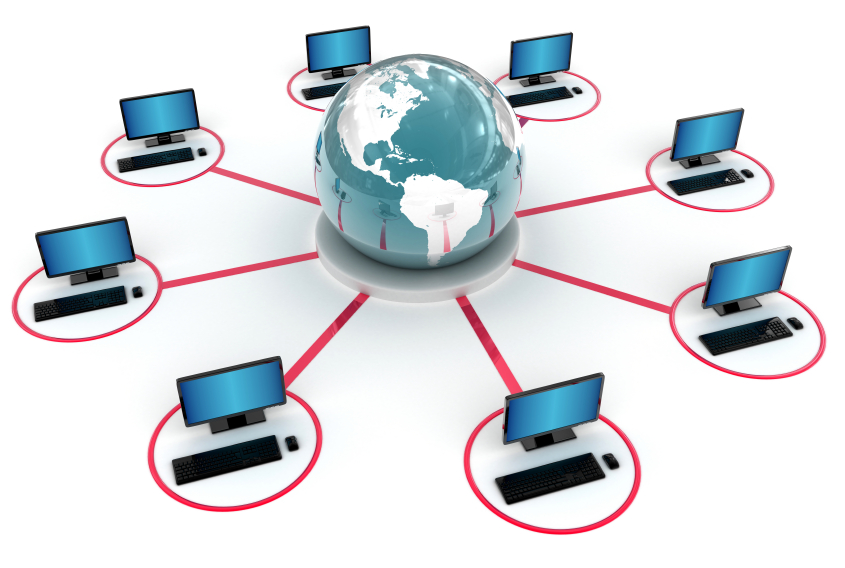
\includegraphics[width = 0.5\textwidth]{images/network.jpg}
\end{center}
\end{frame}

\begin{frame}{Basic SSH}
\begin{itemize}
    \item<1-> Let's try to connect to one of Stanford's \textbf{corn} servers, which are available for general use. Type \emph{ssh your-sunet-id@corn.stanford.edu}
    \item<1-> When prompted for your password, type the password that corresponds to your sunet id. It won't show any characters being typed, just type the password and hit enter. Note: you will probably need to use two-factor authentication, and the timeout is relatively short, have your phone ready
    \item<2-> You should see a welcome screen. If so, congrats, you're connected to a server!
\end{itemize}
\begin{center}\vspace{0em}
\includegraphics[width = 0.5\textwidth]{images/farmshare.png}\end{center}
\end{frame}

\begin{frame}{Basic SSH}
\begin{itemize}
    \item Luckily these servers are running bash as well, so all the commands you've just learned should work here! Try \emph{ls} and see what's around. This is your space on Stanford's servers, you can store documents here, and if you make a Stanford website it will be hosted in the WWW folder. 
    \item Remember, you're no longer on your own computer, so the directory structure here will be different. 
    \item When you're finished, you can type \emph{exit} to close the connection to the server and return to your computer. (But don't do so yet, we're going to keep using it.)
\end{itemize}
\end{frame}

\begin{frame}{A toy website}
\begin{itemize}
    \item<1-> Let's try creating a (very) simple website for you!
    \item<2-> Create a text file called simplewebsite.txt somewhere on your computer, and put some text in it (like "Hello World!"). 
    \item<3-> Now, open a new terminal on your own computer (leave the other terminal with the ssh connection open, we'll go back to it in a bit). \emph{cd} to the directory where you saved simplewebsite.txt.  
\end{itemize}
\begin{center}

\includegraphics[width = 0.5\textwidth]{images/firstwebsite.jpg}
\end{center}
\end{frame}

\begin{frame}{A toy website (cont.)}
\begin{itemize}
    \item<1-> We need to move \emph{simplewebsite.txt} to the Stanford servers. To do that, we'll use the command \emph{scp} (secure copy), which allows you to copy files from/to your local computer to/from a remote one much like you would copy a file on your local computer using \emph{cp} 
    \item<2-> To copy \emph{simplewebsite.txt} to the \emph{$\sim$/WWW} folder on the server, try \emph{scp simplewebsite.txt your-SUNetID@corn.stanford.edu:$\sim$/WWW/} 
    \item<3-> If all went well, you should see the name of the file followed by 100\% (since the file is so small, the transfer will complete very rapidly). 
    \item<3-> If so, try opening your web browser and going to \emph{web.stanford.edu/$\sim$your-SUNetID/simplewebsite.txt} 
    \item<4-> Do you see your file? Congratulations! You've got a very basic website now. You can use the farmshare system to host experiments that you run online, to create a website for yourself so that people can look you up, etc. The process will be similar to this, except that you'll probably be creating html files instead of text files. 
\end{itemize}
\end{frame}

\begin{frame}{Cleaning up the website}
\begin{itemize}
    \item<1-> We left the ssh connection open in the other terminal so we can do something with the file on the server.
    \item<2-> Go ahead and run \emph{ls $\;\sim$/WWW} on the server so you can see \emph{simplewebsite.txt} is there.
    \item<3-> You might not want the world to be able to see this file forever, so change to the \emph{WWW} directory and remove the file.
    \item<4-> Finally, close your connection to the server by typing \emph{exit}.
\end{itemize}
\end{frame}

\section{Wrapping up}

\begin{frame}{Wrapping up}
Bash contains or allows access to many powerful tools, and has many arcane (but useful!) features. Here are a few examples of the things you can do with it that we won't have time to explain to you. If you're interested in more info, talk to us and we'll be happy to provide it!
\end{frame}

\begin{frame}[fragile]{Being lazy (scripts)}
One of the main reasons bash is useful is that bash commands can be saved into scripts that can be reused. For example, here's a simple shell script I wrote to create anonymized data files by replacing participant identifiers in filenames with numbers starting from 0:
\begin{lstlisting}
#!/bin/bash
i=0
for f in data_subject_*.json
do
  cp $f ../anonymized_data/data_subject_${i}.json
  i=$((i+1))
done
\end{lstlisting}
\end{frame}

\begin{frame}{Programming}
The terminal gives you access to programming languages like python, both by running programs directly, and by using \textbf{interpreters}, programs that run in the terminal and allow you to run commands interactively, much as you would in Matlab or R.
\begin{center}
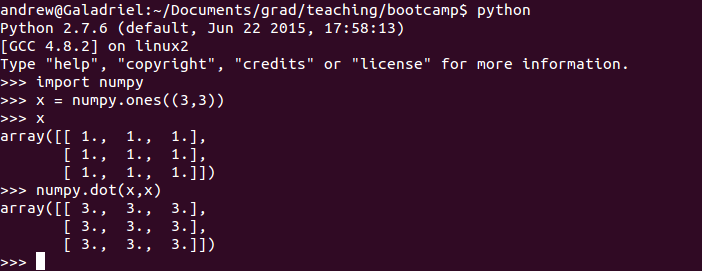
\includegraphics[width = \textwidth]{images/python.png}
\end{center}
\end{frame}

\begin{frame}{Etc.}
Also:
\begin{itemize}
\item Powerful commands for text manipulation (\emph{sed, awk, grep}). Want to find all occurrences of a variable in many different code files and rename it? Want to extract lines from your datafiles that match a certain condition without having to read the files into R? Have a directory full of awful tab-separated datafiles and want to make them comma-separated? These tools can do it. 
\item Streams and piping: make commands work together, do file I/O, etc.   
\item Automation: more system specific, but \emph{cron}, rc files, etc. allow for automation of things like backups, mounting filesystems when you start your computer, or sending reminders to subjects on a schedule.
\item Text-editors like \emph{vim}.
\item Git version control -- You'll learn about this at the later tutorial!
\end{itemize}
\end{frame}

\begin{frame}{Cheatsheet}
\centering
\resizebox{\textwidth}{!}{
\begin{tabular}{|l|p{0.5\textwidth}|}
\hline
\textbf{Command} & \textbf{Effect} \\
\hline
\emph{man command} or \emph{help command} & Get manual/help for a command \\ 
\emph{pwd} & Print working directory \\
\emph{cd dir} & Change working directory to \emph{dir} \\
\emph{ls} & List directory contents \\
\emph{mkdir dir} & Make a new directory called \emph{dir} \\
\emph{rmdir dir} & Remove the directory \emph{dir} permanently \\
\emph{mv source dest} & Move \emph{source} file or folder to \emph{dest} \\
\emph{cp source dest} & Copy \emph{source} file to \emph{dest} (use -r for folders) \\
\emph{rm file} & Remove \emph{file} permanently \\
\emph{ssh user@server} & Connect to \emph{server} as \emph{user} \\
\emph{scp [[user1@]server1:]source [[user2@]server2:]dest} & Copy \emph{source} from \emph{server1} to \emph{dest} on \emph{server2} (if copying to/from your local computer, just omit the server and user parts in that file's path)\\
\hline
\end{tabular}
}
(For a more comprehensive reference see {\color{blue} \url{https://gist.github.com/LeCoupa/122b12050f5fb267e75f}})
\end{frame}

\begin{frame}

\includegraphics[width = \textwidth]{images/thatsallfolks.png}
\end{frame}
\end{document}
